%%%%%%%%%%%%%%%%%%%%%%%%%%%%%%%%%%%%%%%%%%%%%%%%%%%%%%%%%%%%%%%%%%%%%%%%%%%%%%%%

\section{Maintenance}

%%%%%%%%%%%%%%%%%%%%%%%%%%%%%%%%%%%%%%%%%%%%%%%%%%%%%%%%%%%%%%%%%%%%%%%%%%%%%%%%

\begin{frame}[fragile]{EXPLAIN PLAN}

   TODO
   WIP

\begin{toile}
\toileurl{XXXX}
\end{toile}

\end{frame}

%%%%%%%%%%%%%%%%%%%%%%%%%%%%%%%%%%%%%%%%%%%%%%%%%%%%%%%%%%%%%%%%%%%%%%%%%%%%%%%%

\begin{frame}[fragile]{Tâches de maintenance de la base de données}

   La base de données nécessite des opérations de maintenance régulière pour assurer un service optimal.
   Les principales tâches de maintenance sont:
   \begin{itemize}
      \item Les sauvegardes régulières qui permettront de s'en sortir en cas d'accident grave
      \item Les opérations de VACUUM
      \item Les mises à jour des statistiques
      \item Les mises à jour des indexes
      \item La gestion des logs
   \end{itemize}

\begin{toile}
\toileurl{https://www.postgresql.org/docs/15/maintenance.html}
\end{toile}

\end{frame}

%%%%%%%%%%%%%%%%%%%%%%%%%%%%%%%%%%%%%%%%%%%%%%%%%%%%%%%%%%%%%%%%%%%%%%%%%%%%%%%%

\begin{frame}[fragile]{Les opérations de VACUUM}

   Les opérations de VACUUM sont lancées automatiquement par le démon \textsf{autovacuum}. Certains DBAs préfèrent gérer ce process eux-même à partir de tâches de type cron.
   Les raisons principales pour lancer un VACUUM régulier sont:

   \begin{itemize}
      \item récupérer l'espace disque occupé pour des lignes mises à jour ou supprimées
      \item mises à jour des statistiques utilisées par le planificateur de requêtes (query planner)
      \item mises à jour du flag de visibilité pour améliorer la performance des indexes only scan (chapitre Optimisation)
      \item protection contre la perte de données très anciennes causée par la rotation des identifiants de transaction ou de multi-transaction
   \end{itemize}

\begin{toile}
\toileurl{https://www.postgresql.org/docs/15/routine-vacuuming.html}
\end{toile}

\end{frame}

%%%%%%%%%%%%%%%%%%%%%%%%%%%%%%%%%%%%%%%%%%%%%%%%%%%%%%%%%%%%%%%%%%%%%%%%%%%%%%%%

\begin{frame}{Différents type de VACUUM}

   Il existe 2 types de VACUUM:
   \begin{itemize}
      \item le VACUUM standard
      \item le VACUUM FULL 
   \end{itemize}

\end{frame}

%%%%%%%%%%%%%%%%%%%%%%%%%%%%%%%%%%%%%%%%%%%%%%%%%%%%%%%%%%%%%%%%%%%%%%%%%%%%%%%%

\begin{frame}{VACUUM standard}

   \begin{itemize}
      \item Le VACUUM standard peut être lancé en parallèle des commandes SQL (\textbf{SELECT}, \textbf{UPDATE}, \textbf{INSERT} et \textbf{DELETE})
      \item la commande \textbf{ALTER TABLE} ne peut être exécutée sur une table en cours de traitement par le process
      \item le VACUUM génère des I/O très importantes qui diminuent les performances des autres sessions actives
      \item Il est possible de tempérer la charge I/O causée par le VACUUM par l'intermédiaire des paramètres: \textbf{vacuum\_cost\_*} (cf. ~\ref{vacuum-cost})
   \end{itemize}

\end{frame}

%%%%%%%%%%%%%%%%%%%%%%%%%%%%%%%%%%%%%%%%%%%%%%%%%%%%%%%%%%%%%%%%%%%%%%%%%%%%%%%%

\begin{frame}{VACUUM FULL}

   \begin{itemize}
      \item Ce VACUUM récupère plus d'espace disque que le standard.
      \item Il est cependant plus lent
      \item Le VACUUM FULL posse un verrou de type \textbf{ACCESS EXCLUSIVE} sur la table en cours de traitement. Il empêche tout autre traitement d'accéder à la table.
      \item Il est recommandé de privilégier l'utilisation du VACUUM standard
   \end{itemize}

\end{frame}

%%%%%%%%%%%%%%%%%%%%%%%%%%%%%%%%%%%%%%%%%%%%%%%%%%%%%%%%%%%%%%%%%%%%%%%%%%%%%%%%

\begin{frame}{Récupération de l'espace disque}

   \begin{itemize}
      \item Le \textbf{DELETE} ou \textbf{UPDATE} ne supprime pas immédiatement les anciennes versions d'une ligne afin que les process ayant accès à la table ait leur version courante de la ligne jusqu'à la fin de la transaction.
      \item Lorsqu'une version devient obsolète et qu'elle n'est plus utilisée par une session, le VACUUM marque l'espace occupé par la ligne comme disponible pour les prochaines lignes.
      \item Cela permet d'éviter l'explosion de l'espace disque occupé par une table.
      \item L'espace disque n'est donc pas libéré: il devient disponible.
      \item Dans le cas où l'espace disponible se trouve en fin de page et qu'il est facile d'acquérir un verrou de type exclusif, l'espace disque est rendu à l'OS
   \end{itemize}

\end{frame}

%%%%%%%%%%%%%%%%%%%%%%%%%%%%%%%%%%%%%%%%%%%%%%%%%%%%%%%%%%%%%%%%%%%%%%%%%%%%%%%%

\begin{frame}{Récupération de l'espace disque}

   \begin{itemize}
      \item A l'inverse, VACUUM FULL réécrit entièrement la table de manière compacte sans espace vide. Cela réduit la taille occupée par la table mais prend beaucoup de temps.
      \item Durant le VACUUM FULL, l'espace disque de la table double car l'ancienne version est gardée jusqu'à la fin de l'opération
   \end{itemize}

\end{frame}

%%%%%%%%%%%%%%%%%%%%%%%%%%%%%%%%%%%%%%%%%%%%%%%%%%%%%%%%%%%%%%%%%%%%%%%%%%%%%%%%

\begin{frame}{Fréquence de passage du VACUUM}

   \begin{itemize}
      \item La bonne pratique est de lancer un VACUUM standard suffisamment fréquemment pour éviter de lancer le FULL
      \item Le démon autovacuum respecte cette philosophie et n'utilise pas le FULL
      \item L'objectif n'est pas de garder une taille minimale pour les tables
      \item L'objectif est de garder une taille des tables \textbf{stable}
      \item Pour appliquer le VACUUM sur une base de données entière, il est possible d'utiliser \textsf{vacuumdb}
   \end{itemize}

\end{frame}

%%%%%%%%%%%%%%%%%%%%%%%%%%%%%%%%%%%%%%%%%%%%%%%%%%%%%%%%%%%%%%%%%%%%%%%%%%%%%%%%

\begin{frame}{Cas des tables totalement supprimées}

   \begin{itemize}
      \item Lorsqu'une table est entièrement supprimée, la commande \textbf{TRUNCATE} peut être appliquée
      \item TRUNCATE libère automatiquement l'espace disque
      \item \textbf{Limitation:} le TRUNCATE ne respecte les principes du MVCC (vue locale des données pour chaque session)
   \end{itemize}

\end{frame}

%%%%%%%%%%%%%%%%%%%%%%%%%%%%%%%%%%%%%%%%%%%%%%%%%%%%%%%%%%%%%%%%%%%%%%%%%%%%%%%%

\begin{frame}{Cas des tables massivement mises à jour}

   \begin{itemize}
      \item Lorsqu'une table est massivement mise à jour ou supprimée, il peut être intéressant de lancer un VACUUM FULL
      \item Une alternative au VACUUM FULL est la commande \textbf{CLUSTER}
      \item Cette commande réécrit la table en disposant les lignes en suivant l'ordre de l'index d'une colonne
      \item Elle est décrite plus en détail dans la partie optimisation
   \end{itemize}

\end{frame}

%%%%%%%%%%%%%%%%%%%%%%%%%%%%%%%%%%%%%%%%%%%%%%%%%%%%%%%%%%%%%%%%%%%%%%%%%%%%%%%%

\begin{frame}{vacuumdb}

   \begin{itemize}
      \item VACUUM s'applique sur une table.
      \item Pour l'appliquer sur une base de données, il est possible d'utiliser \textbf{vacuumdb}
   \end{itemize}

\begin{toile}
\toileurl{https://www.postgresql.org/docs/15/app-vacuumdb.html}
\end{toile}

\end{frame}

%%%%%%%%%%%%%%%%%%%%%%%%%%%%%%%%%%%%%%%%%%%%%%%%%%%%%%%%%%%%%%%%%%%%%%%%%%%%%%%%

\begin{frame}{Mise à jour des statistiques du planificateur de requêtes}

   \begin{itemize}
      \item Le planificateur de requêtes s'appuie sur les statistiques collectées sur les tables
      \item La commande \textbf{ANALYZE} exécute la génération de statistiques sur une table
      \item L'ANALYZE est également une option de la commande VACUUM. De cette manière, les 2 opérations sont lancées en parallèle sur la table.
      \item L'ANALYZE est également une option du démon \textbf{autovacuum}
      \item Dans le cas où l'administrateur système sait que les mises à jour de la table n'affecte pas les statistiques, il est possible de gérer l'ANALYZE manuellement.
      \item \textbf{Les mises à jour dans les partitions de table ou les tables enfants ne provoquent d'ANALYZE automatique des tables parentes.}
      \item Pour cela, il est nécessaire de lancer l'ANALYZE manuellement sur les tables parentes.
   \end{itemize}

\begin{toile}
\toileurl{https://www.postgresql.org/docs/15/sql-vacuum.html}
\end{toile}

\end{frame}

%%%%%%%%%%%%%%%%%%%%%%%%%%%%%%%%%%%%%%%%%%%%%%%%%%%%%%%%%%%%%%%%%%%%%%%%%%%%%%%%

\begin{frame}{Cas des tables fréquemment mises à jour}

   \begin{itemize}
      \item En fonction de la répartition des valeurs de données dans une colonne, il peut être intéressant ou non de lancer la commande ANALYZE
      \item Pour des données ayant une plage de valeurs importante, l'ANALYZE est intéressant
      \item Dans le cas inverse, il n'est pas nécessaire dans le lancer
      \item L'ANALYZE peut être être restreint à une \textbf{colonne}. Particulièrement, celles impliquées dans les clauses WHERE avec une répartition de valeurs extrêmement irrégulière.
      \item En pratique, il s'avère plus efficace d'appliquer l'ANALYZE à la base de données
   \end{itemize}

\end{frame}

%%%%%%%%%%%%%%%%%%%%%%%%%%%%%%%%%%%%%%%%%%%%%%%%%%%%%%%%%%%%%%%%%%%%%%%%%%%%%%%%

\begin{frame}{Qualité des statistiques}

   Pour augmenter l'échantillonage de l'ANALYZE, il est possible d'utiliser 2 paramètres:
   \begin{itemize}
      \item \textbf{default\_statistic\_target}. Par défaut, 100. La base de données sera impactée
      \item \textbf{ALTER TABLE SET STATISTICS}. Seule la table sera impactée.
   \end{itemize}

\begin{toile}
\toileurl{https://www.postgresql.org/docs/15/runtime-config-query.html\#GUC-DEFAULT-STATISTICS-TARGET}
\end{toile}

\end{frame}

%%%%%%%%%%%%%%%%%%%%%%%%%%%%%%%%%%%%%%%%%%%%%%%%%%%%%%%%%%%%%%%%%%%%%%%%%%%%%%%%

\begin{frame}{Mise à jour du tableau de visibilité}

\begin{itemize}
   \item La table de visibilité de chaque page indique si une page de données est visible à toutes ltransactions actives.
   \item Si elle a été modifiée par une session et est en attente de flush vers le disque (dirty page), elle sera traitée par le VACUUM.
   \item Sinon elle ne sera pas traitée par le VACUUM.
   \item Le module \textbf{pg\_visibility} permet de visualiser les informations stockées dans la table de visibilité.
   \item La table de visibilité est utilisée pour les index-only scans pour éviter à l'index de rafraîchir les données qu'il embarque.
\end{itemize}

\begin{toile}
\toileurl{https://www.postgresql.org/docs/15/storage-vm.html}
\toileurl{https://www.postgresql.org/docs/15/pgvisibility.html}
\end{toile}
   
\end{frame}

%%%%%%%%%%%%%%%%%%%%%%%%%%%%%%%%%%%%%%%%%%%%%%%%%%%%%%%%%%%%%%%%%%%%%%%%%%%%%%%%

\begin{frame}{Prévention des erreurs causées par la rotation des identifiants de transaction}

\begin{itemize}
   \item Chaque transaction (XID) a un identifiant stocké sur un entier de 32 bits
   \item Cela autorise $2^{32}$ transactions
   \item Au bout de ce nombre de transaction, le compteur XID repasse à 0
   \item Les transactions qui étaient dans le passé se retrouvent dans le futur
   \item Pour prévenir ce type de situation, PostgreSQL utilise un identifiant spécial \textbf{FrozenTransactionId}
   \item Cet identifiant est antérieur à toute valeur de XID
   \item C'est le rôle du VACUUM de positionner cet identifiant de transaction sur la ligne
\end{itemize}

\end{frame}

%%%%%%%%%%%%%%%%%%%%%%%%%%%%%%%%%%%%%%%%%%%%%%%%%%%%%%%%%%%%%%%%%%%%%%%%%%%%%%%%

\begin{frame}{Rayon de $2^{31}$ pour chaque XID}

\begin{itemize}
   \item D'après ce qui a été dit précédemment chaque XID voit:
   \begin{itemize}
      \item au maximum $2^{31}$ transactions plus anciennes que lui
      \item et au maximum $2^{31}$ transactions plus récente que lui
   \end{itemize}
\end{itemize}

\end{frame}

%%%%%%%%%%%%%%%%%%%%%%%%%%%%%%%%%%%%%%%%%%%%%%%%%%%%%%%%%%%%%%%%%%%%%%%%%%%%%%%%

\begin{frame}{VACUUM \textbf{agressif}}

\begin{itemize}
   \item le VACUUM s'appuie sur la table de visibilité pour savoir s'il est nécessaire de traiter la table et supprimer les versions obsolètes des lignes
   \item Il est cependant parfois nécessaire de geler les XID et MXID d'un certain âge
   \item Cette opération s'appelle le VACUUM \textbf{agressif}
\end{itemize}

\end{frame}

%%%%%%%%%%%%%%%%%%%%%%%%%%%%%%%%%%%%%%%%%%%%%%%%%%%%%%%%%%%%%%%%%%%%%%%%%%%%%%%%

\begin{frame}{Age d'une ligne}

\begin{itemize}
   \item Ma compréhension de la documentation m'incite à dire que l'âge d'une ligne a pour formule:
      \begin{itemize}
      \item si $XID courant > XID ligne, age = XID courant - XID ligne$
      \item sinon, $age = XID courant - XID ligne + 2^{31}$
      \end{itemize}
   \item Une ligne ne sera jamais plus \textit{âgée} que $2^{31} = 2$ millions transactions
   \item A partir d'un certain âge paramétrable, son XID est gelé en FrozenTransactionId
\end{itemize}

\end{frame}

%%%%%%%%%%%%%%%%%%%%%%%%%%%%%%%%%%%%%%%%%%%%%%%%%%%%%%%%%%%%%%%%%%%%%%%%%%%%%%%%

\begin{frame}{\textbf{vacuum\_freeze\_min\_age}}

\begin{itemize}
   \item \textbf{vacuum\_freeze\_min\_age} indique le nombre de transactions \textbf{"vues par le XID de la ligne"} au-delà duquel VACUUM envisage de traiter une \textbf{ligne} de table pour geler son XID
   \item Il correspond à l'âge minimum d'une ligne pour être éligible au VACUUM agressif
   \item Une valeur trop basse de ce paramètre déclenche le gel \textsf{potentiellement inutile} d'une ligne avec le risque qu'elle soit dégelée en cas de modification
   \item Une valeur trop haute de ce paramètre augmente le nombre de transactions nécessaires avant que cette \textbf{ligne} de table puisse être traitée à nouveau par le VACUUM
   \item Valeur comprise entre 0 et $10^{9}$. Par défaut, $50*10^{6}$ transactions.
   \item Valeur automatiquement cappée à $\textbf{autovacuum\_freeze\_max\_age}/2$
\end{itemize}

\begin{toile}
\toileurl{https://www.postgresql.org/docs/15/runtime-config-client.html\#GUC-VACUUM-FREEZE-MIN-AGE}
\end{toile}

\end{frame}

%%%%%%%%%%%%%%%%%%%%%%%%%%%%%%%%%%%%%%%%%%%%%%%%%%%%%%%%%%%%%%%%%%%%%%%%%%%%%%%%

\begin{frame}{Age d'une table - \textbf{vacuum\_freeze\_table\_age}}

\begin{itemize}
   \item Le serveur applique un VACUUM \textbf{agressif} à la table lorsque \textbf{vacuum\_freeze\_table\_age} - \textbf{pg\_class.relfrozenxid} est positif
   \item Lorsque $\textbf{vacuum\_freeze\_table\_age} = 0$, un VACUUM agressif est systématiquement appliqué
   \item \textbf{pg\_class.relfrozenxid} est le niveau du XID en dessous duquel tous les XID de la table ont été gelés
   \item En résumé, il correspond au XID le plus vieux de la table et indique en somme "l'âge" de la table
   \item Valeur par défaut: $150 * 10^6$ transactions
\end{itemize}

\begin{toile}
\toileurl{https://www.postgresql.org/docs/15/catalog-pg-class.html}
\end{toile}

\end{frame}

%%%%%%%%%%%%%%%%%%%%%%%%%%%%%%%%%%%%%%%%%%%%%%%%%%%%%%%%%%%%%%%%%%%%%%%%%%%%%%%%

\begin{frame}{\textbf{autovacuum} et \textbf{vacuum\_freeze\_min\_age}}

\begin{itemize}
   \item la durée maximale qu'une table ne soit pas traitée par un VACUUM agressif est: $2^{31} - \textbf{vacuum\_freeze\_min\_age}$
   \item La valeur de \textbf{vacuum\_freeze\_min\_age} est stockée au passage du dernier VACUUM agressif
   \item La fréquence du passage de l'\textbf{autovacuum} est environ toutes les $\textbf{autovacuum\_freeze\_max\_age} - \textbf{vacuum\_freeze\_min\_age}$ transactions.
   \item Pour empêcher la perte de données, il est déclenché même si \textbf{autovacuum\_freeze\_max\_age} n'est pas positionné
   \item La limite maximale posée par PostgreSQL est: $\textbf{vacuum\_freeze\_table\_age} = 0.95 * \textbf{autovacuum\_freeze\_max\_age}$
\end{itemize}

\end{frame}

%%%%%%%%%%%%%%%%%%%%%%%%%%%%%%%%%%%%%%%%%%%%%%%%%%%%%%%%%%%%%%%%%%%%%%%%%%%%%%%%

\begin{frame}{Paramètre \textbf{autovacuum\_freeze\_max\_age}}

\begin{itemize}
   \item Une valeur plus élevée de \textbf{vacuum\_freeze\_table\_age} est inutile (car le VACUUM agressif sera déclenché par \textbf{autovacuum\_freeze\_max\_age})
   \item Une valeur moins élevée de \textbf{vacuum\_freeze\_table\_age} déclenchera des VACUUM agressifs plus fréquents
   \item Le seul inconvénient d'augmenter \textbf{autovacuum\_freeze\_max\_age} entraîne un espace disque plus important occupé par les répertoires: 
      \begin{itemize}
         \item \textbf{pg\_xact}: Statut des commits
         \item \textbf{pg\_commit\_ts}: Timestamp des commits si cette fonctionnalité est activée
      \end{itemize}
   \item Valeur par défaut: $200*10^{6}$ 
\end{itemize}

\begin{toile}
\toileurl{https://www.postgresql.org/docs/15/runtime-config-autovacuum.html\#GUC-AUTOVACUUM-FREEZE-MAX-AGE}
\end{toile}

\end{frame}

%%%%%%%%%%%%%%%%%%%%%%%%%%%%%%%%%%%%%%%%%%%%%%%%%%%%%%%%%%%%%%%%%%%%%%%%%%%%%%%%

\begin{frame}{Schéma récapitulatif}

\begin{figure}
\begin{center}
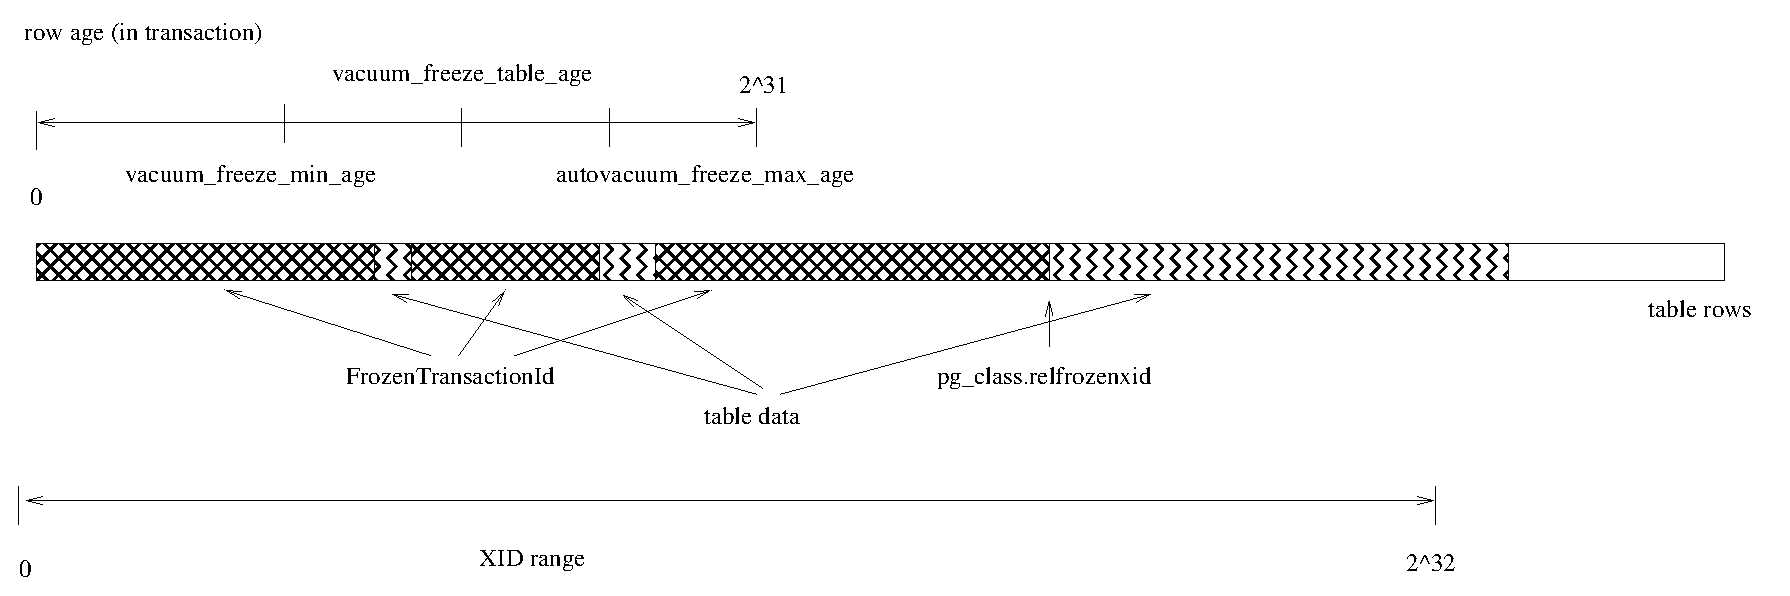
\includegraphics[angle=0, width=\textwidth]{images/xid_freeze.eps}
\end{center}
\end{figure}

\end{frame}

%%%%%%%%%%%%%%%%%%%%%%%%%%%%%%%%%%%%%%%%%%%%%%%%%%%%%%%%%%%%%%%%%%%%%%%%%%%%%%%%

\begin{frame}{Tables de suivi des XID}

\begin{itemize}
   \item Les données sur les XIDs sont stockées dans les table pg\_class et pg\_database
   \item La colonne pg\_class.relfrozenxid indique le plus ancien XID non gelé de la table
   \item Cette colonne est mise à jour par la dernière opération de VACUUM agressif réussie
   \item Au niveau base de données, la colonne pg\_database.datfrozenxid indique le min de tous les pg\_class.relfrozenxid
\end{itemize}

\end{frame}

%%%%%%%%%%%%%%%%%%%%%%%%%%%%%%%%%%%%%%%%%%%%%%%%%%%%%%%%%%%%%%%%%%%%%%%%%%%%%%%%

\begin{frame}[fragile]{Requêtes SQL pour le suivi des XID}

\begin{tiny}
\begin{Verbatim}[commandchars=\\\{\}]
SELECT c.oid::regclass as table_name,
       greatest(age(c.relfrozenxid),age(t.relfrozenxid)) as age
FROM pg_class c
LEFT JOIN pg_class t ON c.reltoastrelid = t.oid
WHERE c.relkind IN ('r', 'm');

SELECT datname, age(datfrozenxid) FROM pg_database;
\end{Verbatim}
\end{tiny}

\begin{itemize}
   \item La colonne age indique le nombre de transactions entre le XID courant et celui du cutoff du VACUUM agressif
   \item relkind = 'r': table ordinaire
   \item relkind = 'm': vue matérialisée
\end{itemize}

\begin{toile}
\toileurl{https://www.postgresql.org/docs/15/catalog-pg-class.html}
\end{toile}

\end{frame}

%%%%%%%%%%%%%%%%%%%%%%%%%%%%%%%%%%%%%%%%%%%%%%%%%%%%%%%%%%%%%%%%%%%%%%%%%%%%%%%%

\begin{frame}{Logs de suivi des VACUUM}

\begin{itemize}
   \item Lorsque l'option \textbf{VERBOSE} de VACUUM est activée, certaines statistiques de la table sont affichées.
   \item L'évolution des champs \textbf{relfrozenxid} et \textbf{relminmxid} est mentionné
   \item Le même niveau de détails de log est activé lorsque l'option \textbf{log\_autovacuum\_min\_duration} a une valeur différente de -1
   \item Valeur par défaut de l'option $\textbf{log\_autovacuum\_min\_duration} = 10$ minutes
   \item Cette option est pratique car elle permet de surveiller l'activité de l'autovacuum
\end{itemize}

\end{frame}

%%%%%%%%%%%%%%%%%%%%%%%%%%%%%%%%%%%%%%%%%%%%%%%%%%%%%%%%%%%%%%%%%%%%%%%%%%%%%%%%

\begin{frame}{Le champ relminmxid}

\begin{itemize}
   \item To translate
   \item All multixact IDs before this one have been replaced by a transaction ID in this table. This is used to track whether the table needs to be vacuumed in order to prevent multixact ID wraparound or to allow pg\_multixact to be shrunk. Zero (InvalidMultiXactId) if the relation is not a table.
\end{itemize}

\begin{toile}
\toileurl{https://www.postgresql.org/docs/15/catalog-pg-class.html}
\end{toile}

\end{frame}

%%%%%%%%%%%%%%%%%%%%%%%%%%%%%%%%%%%%%%%%%%%%%%%%%%%%%%%%%%%%%%%%%%%%%%%%%%%%%%%%

\begin{frame}[fragile]{En cas d'échec de l'autovacuum}

\begin{itemize}
   \item En cas d'échec de l'autovacuum, le serveur émet le warning suivant avant la limite $2^{32} - 40$ millions de transactions:
\begin{tiny}
\begin{Verbatim}[commandchars=\\\{\}]
WARNING:  database "mydb" must be vacuumed within 39985967 transactions
HINT:  To avoid a database shutdown, execute a database-wide VACUUM in that database.
\end{Verbatim}
\end{tiny}
   \item Un VACUUM lancé par un \textbf{super utilisateur} devrait résoudre le problème
   \item Les droits \textbf{super utilisateur} sont nécessaires pour modifier le champ \textbf{datfrozenxid}
   \item Si le DBA ignore les avertissements, le serveur s'arrête et refuse toute nouvelle transaction avant la limite $2^{32} - 3$ millions de transactions:
\begin{tiny}
\begin{Verbatim}[commandchars=\\\{\}]
ERROR:  database is not accepting commands to avoid wraparound data loss in database "mydb"
HINT:  Stop the postmaster and vacuum that database in single-user mode.
\end{Verbatim}
\end{tiny}
   \item Dans ce cas, il devient nécessaire de lancer le serveur en mode single-user
\end{itemize}

\end{frame}

%%%%%%%%%%%%%%%%%%%%%%%%%%%%%%%%%%%%%%%%%%%%%%%%%%%%%%%%%%%%%%%%%%%%%%%%%%%%%%%%

\begin{frame}[fragile]{Démarrage du serveur PostgreSQL en mode single-user}

\begin{itemize}
   \item Pour démarrer le serveur en mode single-user, lancer la commande suivante:
\begin{tiny}
\begin{Verbatim}[commandchars=\\\{\}]
   postgres --single -D /usr/local/pgsql/data other-options my_database
\end{Verbatim}
\end{tiny}
   \item Dans ce mode, le serveur n'applique pas les mesures de sécurité pour éteindre le process en cas de "danger"
   \item A ce moment, il devient possible de lancer le VACUUM FREEZE
\end{itemize}

\begin{toile}
\toileurl{https://www.postgresql.org/docs/15/app-postgres.html}
\end{toile}

\end{frame}

%%%%%%%%%%%%%%%%%%%%%%%%%%%%%%%%%%%%%%%%%%%%%%%%%%%%%%%%%%%%%%%%%%%%%%%%%%%%%%%%

\begin{frame}{Multi-transactions et repli des identifiants de transactions}

\begin{itemize}
   \item Il est possible qu'une ligne de table soit verrouillé par plusieurs transactions
   \item Les identifiants de transactions multiples sont stockés dans le répertoire \textbf{pg\_multixact}
   \item Comme pour les transactions classiques, ils sont stockées sur 32 bits et varient entre 0 et $2^{32}$
   \item Les seuils de traitement d'une ligne et d'une table sont respectivement \textbf{vacuum\_multixact\_freeze\_min\_age} et \textbf{vacuum\_multixact\_freeze\_table\_age}
   \item L'indicateur d'âge d'une table pour les multi-transactions est: \textbf{pg\_class.relminmxid}
   \item De manière similaire,  toute table ayant l'âge \textbf{autovacuum\_multixact\_freeze\_max\_age} pour ses multitransactions, sera traitée par un VACUUM agressif

\end{itemize}

\end{frame}

%%%%%%%%%%%%%%%%%%%%%%%%%%%%%%%%%%%%%%%%%%%%%%%%%%%%%%%%%%%%%%%%%%%%%%%%%%%%%%%%

\begin{frame}{Le démon \textbf{autovacuum}}

\begin{itemize}
   \item L'autovacuum lance automatiquement le VACUUM et l'NALAYZE (collecte de statistiques) sur chaque table
   \item Par défaut, le paramètre \textbf{track\_counts} = on. Il est utilisé par l'autovacuum pour suivre l'activité de la base de données et se déclencher au moment opportun
   \item Le démon autovacuum se décline en plusieurs process:
   \begin{itemize}
      \item l'\textbf{autovacuum launcher} en charge de démarrer l'\textbf{autovacuum worker} pour chaque base de données
      \item le launcher démarre un work tous les \textbf{autovacuum\_naptime} secondes pour chaque base de données
   \end{itemize}
   \item un work sera donc lancé tous les \text{autovacuum\_naptime}/N secondes s'il y a N bases de données
   \item La limite est de \textbf{autovacuum\_max\_workers} worker par base de données

\end{itemize}

\end{frame}

%%%%%%%%%%%%%%%%%%%%%%%%%%%%%%%%%%%%%%%%%%%%%%%%%%%%%%%%%%%%%%%%%%%%%%%%%%%%%%%%

\begin{frame}{Le paramètre \textbf{autovacuum\_max\_workers}}

\begin{itemize}
   \item Si le nombre de bases de données est supérieur à autovacuum\_max\_workers, la prochaine base de données sera traité sitôt que le worker aura fini.
   \item Les worker ne sont pas inclus dans les limites \textbf{max\_connections} or \textbf{superuser\_reserved\_connections}.

\end{itemize}

\begin{toile}
\toileurl{https://www.postgresql.org/docs/15/runtime-config-autovacuum.html}
\end{toile}

\end{frame}

%%%%%%%%%%%%%%%%%%%%%%%%%%%%%%%%%%%%%%%%%%%%%%%%%%%%%%%%%%%%%%%%%%%%%%%%%%%%%%%%

\begin{frame}[fragile]{A quel moment autovacuum se déclenche - modifications/suppressions}

\begin{itemize}
   \item Lorsqu'une table a une valeur \textbf{relfrozenxid} plus âgée que \textbf{autovacuum\_freeze\_max\_age}
   \item Lorsque le nombre de relations de la table (modifiées ou supprimées depuis le dernier VACUUM) atteint le seuil suivant:
\begin{tiny}
\begin{Verbatim}[commandchars=\\\{\}]
vacuum threshold = vacuum base threshold + vacuum scale factor * number of tuples
\end{Verbatim}
\end{tiny}
   \item avec vacuum base threshold = autovacuum\_vacuum\_threshold et vacuum scale factor = autovacuum\_vacuum\_scale\_factor
   \item le nombre de tuples est fourni par pg\_class.reltuples

\end{itemize}

\end{frame}

%%%%%%%%%%%%%%%%%%%%%%%%%%%%%%%%%%%%%%%%%%%%%%%%%%%%%%%%%%%%%%%%%%%%%%%%%%%%%%%%

\begin{frame}[fragile]{A quel moment autovacuum se déclenche - insertions}

\begin{itemize}
   \item Lorsque le nombre de relations de la table (inserées depuis le dernier VACUUM) atteint le seuil suivant:
\begin{tiny}
\begin{Verbatim}[commandchars=\\\{\}]
vacuum insert threshold = vacuum base insert threshold + vacuum insert scale factor * number of tuples
\end{Verbatim}
\end{tiny}
   \item avec vacuum base insert threshold = autovacuum\_vacuum\_insert\_threshold et vacuum scale factor = autovacuum\_vacuum\_insert\_scale\_factor
   \item le nombre de tuples est fourni par pg\_class.reltuples
   \item Pour une table modifiée principalement par \textbf{INSERT} et peu par \textbf{UPDATE} ou \textbf{DELETE}, il est intéressant de baisser le seuil \textbf{autovacuum\_freeze\_min\_age} pour alléger la charge des prochains VACUUM (\textit{avec un risque de dégel peu élevé})

\end{itemize}

\end{frame}

%%%%%%%%%%%%%%%%%%%%%%%%%%%%%%%%%%%%%%%%%%%%%%%%%%%%%%%%%%%%%%%%%%%%%%%%%%%%%%%%

\begin{frame}[fragile]{A quel moment autovacuum réalise un ANALYZE}

\begin{itemize}
\begin{tiny}
\begin{Verbatim}[commandchars=\\\{\}]
analyze threshold = analyze base threshold + analyze scale factor * number of tuples
\end{Verbatim}
\end{tiny}
   \item Le seuil d'ANALYZE est comparé avec le nombre de lignes en INSERT, DELETE ou UPDATE depuis le dernier ANALYZE
   \item avec analyze base threshold = \textbf{autovacuum\_analyze\_threshold} et analyze scale factor = \textbf{autovacuum\_analyze\_scale\_factor}

\end{itemize}

\end{frame}

%%%%%%%%%%%%%%%%%%%%%%%%%%%%%%%%%%%%%%%%%%%%%%%%%%%%%%%%%%%%%%%%%%%%%%%%%%%%%%%%

\begin{frame}[fragile]{Limites de l'autovacuum}

\begin{itemize}
   \item Les tables partitionnées ne sont pas traitées par l'autovacuum
   \item Les statistiques sont collectés manuellement en lançant un ANALYZE manuel à l'initialisation de la table et après chaque changement significatif
   \item Les tables temporaires ne sont pas accessibles par l'autovacuum
   \item Elles nécessitent un traitement manuel de l'ANALYZE et VACUUM en passant par des commandes SQL
   \item Les paramètres de l'autovacuum sont définis dans \textbf{postgresql.conf}. Cependant, il est possible de les surcharger directement à la définition de la table

\end{itemize}

\begin{tiny}
\begin{toile}
\toileurl{https://www.postgresql.org/docs/15/sql-createtable.html\#SQL-CREATETABLE-STORAGE-PARAMETERS}
\end{toile}
\end{tiny}

\end{frame}

%%%%%%%%%%%%%%%%%%%%%%%%%%%%%%%%%%%%%%%%%%%%%%%%%%%%%%%%%%%%%%%%%%%%%%%%%%%%%%%%

\begin{frame}{Répartition de la charge du VACUUM par les facteurs de coûts}

\begin{itemize}
   \item Durant les opérations de VACUUM ou d'ANALYZE, les opérations I/O peuvent être pénalisantes pour les autres opérations du serveur
   \item Lors de l'exécution des commandes VACUUM et ANALYZE, le serveur garde une trace des coûts I/O engendrés par ces opérations et réalise une accumulation de ces coûts.
   \item Il est possible pour l'administrateur de définir un seuil d'accumulation d'I/O à partir duquel le VACUUM rentre en sommeil et les coûts sont remis à 0.
   \item Par défaut, cette fonctionnalité est \textbf{désactivée} pour les opérations manuelles. Pour l'activer, il est nécessaire de positionner le paramètre \textbf{vacuum\_cost\_delay} à une valeur différente de zéro.
   \item Le seuil est défini par le paramètre \textbf{vacuum\_cost\_limit}. Valeur par défaut 200.
   \item La durée de sommeil du process VACUUM en millisecondes est: \textbf{vacuum\_cost\_delay}. Valeur par défaut 0.

\end{itemize}

\begin{tiny}
\begin{toile}
\toileurl{https://www.postgresql.org/docs/15/runtime-config-resource.html\#RUNTIME-CONFIG-RESOURCE-VACUUM-COST}
\end{toile}
\end{tiny}

\end{frame}

%%%%%%%%%%%%%%%%%%%%%%%%%%%%%%%%%%%%%%%%%%%%%%%%%%%%%%%%%%%%%%%%%%%%%%%%%%%%%%%%

\begin{frame}[fragile]{Comment est calculé le coût du VACUUM}
\label{vacuum-cost}

\begin{itemize}
   \item Les différents critères utilisés pour calculer le coût d'un VACUUM sont:
   \begin{itemize}
      \item \textbf{vacuum\_cost\_page\_hit}: Coût de verrouillage du buffer, recherche et scan de la page associée. Valeur par défaut: 1
      \item \textbf{vacuum\_cost\_page\_miss}: Coût de verrouillage, récupération de la page depuis le disque et scan. Valeur par défaut: 2
      \item \textbf{vacuum\_cost\_page\_dirty}: Coût de modification d'une page par le VACUUM (gel, table de visibilité, \ldots). I/O nécessaire pour écrire la page en disque. Valeur par défaut: 20
   \end{itemize}
   \item Ces paramètres de coût s'appliquent sur l'ensemble des workers et sont répartis sur cet ensemble.
   \item Cependant, lorsqu'un worker traite une table ayant positionné \textbf{autovacuum\_vacuum\_cost\_delay} ou \textbf{autovacuum\_vacuum\_cost\_limit}, les coûts induits par ce traitement ne sont pas inclus dans les coûts globaux.
\end{itemize}

\begin{tiny}
\begin{toile}
\toileurl{https://www.postgresql.org/docs/15/runtime-config-resource.html\#RUNTIME-CONFIG-RESOURCE-VACUUM-COST}
\end{toile}
\end{tiny}

\end{frame}

%%%%%%%%%%%%%%%%%%%%%%%%%%%%%%%%%%%%%%%%%%%%%%%%%%%%%%%%%%%%%%%%%%%%%%%%%%%%%%%%

\begin{frame}{Traitement des verrous par l'autovacuum}

\begin{itemize}
   \item Les workers autovacuum ne bloquent pas les autres process en général
   \item Si un process essaie d'acquérir un verrou de type \textbf{SHARE UPDATE EXCLUSIVE} qui entre en collision avec l'autovacuum, l'autovacuum est interrompu
   \item Dans le cas où l'autovacuum démarre pour prévenir le pli des identifiants de transaction (XID wraparound), celui-ci n'est pas interruptible
   \item La requête lancée par l'autovacuum dans ce cas se termine par la chaîne "(to prevent wraparound)" dans la vue pg\_stat\_activity
   \item Le lancement fréquent de commandes qui réclame des verrous de type \textbf{SHARE UPDATE EXCLUSIVE} empêche l'autovacuum de se terminer systématiquement
\end{itemize}

\end{frame}

%%%%%%%%%%%%%%%%%%%%%%%%%%%%%%%%%%%%%%%%%%%%%%%%%%%%%%%%%%%%%%%%%%%%%%%%%%%%%%%%

\begin{frame}{La réindexation}

\begin{itemize}
   \item Lorsque des clés de l'index sont regulièrement supprimées, il est intéressant de lancer la commande \textbf{REINDEX}
   \item Elle permet de récupérer l'espace non utilisé et améliore légèrement l'accès aux index
   \item REINDEX réorganise les clés de l'index de manière adjacente pour permettre un accès optimal
   \item L'occupation de l'espace disque par les indexes non B-tree n'est pas très bien maîtrisée.
   \item Il est important de surveiller l'espace disque occupé par les index
   \item REINDEX pose par défaut un verrou de type \textbf{ACCESS EXCLUSIVE} sur la table en cours d'indexation.
   \item Il est impossible de modifier la table pendant ce type de réindexation
   \item Le process de réindexation renseigne la table \textbf{pg\_stat\_progress\_create\_index} pendant son exécution

\end{itemize}

\begin{toile}
\toileurl{https://www.postgresql.org/docs/15/routine-reindex.html}
\end{toile}

\end{frame}

%%%%%%%%%%%%%%%%%%%%%%%%%%%%%%%%%%%%%%%%%%%%%%%%%%%%%%%%%%%%%%%%%%%%%%%%%%%%%%%%

\begin{frame}{La réindexation concurrente}

\begin{itemize}
   \item La réindexation concurrente est activée avec l'option \textbf{CONCURRENTLY}
   \item Elle permet la modification de la table en cours de réindexation
   \item Elle est plus gourmande en CPU et I/O car l'index est généré en 2 passes:  
   \begin{itemize}
      \item Une première passe pour scanner la table et regénérer un index temporaire
      \item Cet index devient disponible pour l'ajout de clés
      \item Une deuxième passe pour récupérer les clés générées pendant la première phase
   \end{itemize}


\end{itemize}

\begin{toile}
\toileurl{https://www.postgresql.org/docs/15/sql-reindex.html}
\end{toile}

\end{frame}

%%%%%%%%%%%%%%%%%%%%%%%%%%%%%%%%%%%%%%%%%%%%%%%%%%%%%%%%%%%%%%%%%%%%%%%%%%%%%%%%

\begin{frame}[fragile]{Troubleshooting de la réindexation concurrente}

\begin{itemize}
   \item En cas d'erreur de rebuild de l'index, la commande \textbackslash d appliquée à la table permet de vérifier l'état des index de la table:
\begin{tiny}
\begin{Verbatim}[commandchars=\&\`\!]
   postgres=# \d tab
       Table "public.tab"
 Column |  Type   | Modifiers
--------+---------+-----------
 col    | integer |
Indexes:
    "idx" btree (col)
    "idx_ccnew" btree (col) INVALID
\end{Verbatim}
\end{tiny}
   \item Dans le cas présent, l'index est à l'état invalide
   \item Il est suffixé par \textbf{ccnew}, il correspond à l'index temporaire créé à la première passe
   \item Il suffit de le supprimer avec la commande \commande{DROP INDEX} et de le recréer avec \commande{REINDEX CONCURRENTLY}
   \item S'il est suffixé par \textbf{ccold}, il correspond à l'index original qui est maintenant obsolète
   \item Il suffit de le supprimer avec la commande \commande{DROP INDEX}

\end{itemize}

\end{frame}

%%%%%%%%%%%%%%%%%%%%%%%%%%%%%%%%%%%%%%%%%%%%%%%%%%%%%%%%%%%%%%%%%%%%%%%%%%%%%%%%

\begin{frame}[fragile]{Limites de la réindexation concurrente}

\begin{itemize}
   \item Il est possible d'appliquer plusieurs \textbf{REINDEX} sur d'autres index de la table en parallèle
   \item Ce n'est pas possible avec \textbf{REINDEX CONCURRENTLY}
   \item \textbf{REINDEX CONCURRENTLY} n'est pas utilisable dans une transaction alors que \textbf{REINDEX} est utilisable dans une transaction
   \item \textbf{REINDEX SYSTEM} n'est pas utilisable avec l'option \textbf{CONCURRENTLY}
   \item L'option \textbf{CONCURRENTLY} ne peut pas être utilisable sur un index de type contrainte d'exclusion. Ce type d'index peut être réindexé sans l'option \textbf{CONCURRENTLY}

\end{itemize}


\begin{tiny}
\begin{toile}
\toileurl{https://www.postgresql.org/docs/current/ddl-partitioning.html\#DDL-PARTITIONING-CONSTRAINT-EXCLUSION}
\end{toile}
\end{tiny}

\end{frame}

%%%%%%%%%%%%%%%%%%%%%%%%%%%%%%%%%%%%%%%%%%%%%%%%%%%%%%%%%%%%%%%%%%%%%%%%%%%%%%%%

\begin{frame}[fragile]{Exercices}

   \begin{itemize}
\item VACUUM
\item VACUUM FULL après DELETE pour vérifier récuperation espace disque
\item Modifier freeze\_min\_age et freeze\_table\_age
\item VACUUM FREEZE
\item relfrozenxid
\item reindexation
   \end{itemize}

\end{frame}

%%%%%%%%%%%%%%%%%%%%%%%%%%%%%%%%%%%%%%%%%%%%%%%%%%%%%%%%%%%%%%%%%%%%%%%%%%%%%%%%

\begin{frame}[fragile]{Tests de vérification de la bonne santé de la base}

   TODO
   WIP

\begin{toile}
\toileurl{https://bucardo.org/check\_postgres/}
\end{toile}

\end{frame}

%%%%%%%%%%%%%%%%%%%%%%%%%%%%%%%%%%%%%%%%%%%%%%%%%%%%%%%%%%%%%%%%%%%%%%%%%%%%%%%%
